\chapter{Create a Grid and visualise the associated Mesh}
In this section, we show how to create a grid with \Atlas 
and successively how to generate a mesh from the grid, in 
order to visualise it in Gmsh.
% 
\begin{notebox}
With the term \textit{grid} we intend a list of points without 
any specific connectivity rule, while with the \textit{mesh} 
we intend an object composed by elements and specific connectivity 
rules.
\end{notebox}
%
There can be different types of grids depending on the requirements 
and constraints one might have. 

In this section we will focus on two types of grids, Gaussian 
and reduced Gaussian grids, and we will show how to create them 
for both C++ and Fortran.



\section{C++ version}
\subsection{Gaussian Grids}
A Gaussian grid is defined just by the number of latitudes in one 
hemisphere. It is in fact constructed in a symmetric way with respect 
to the equator and is formed by a number of longitudinal points equal 
to:
%
\begin{equation}
N_{lon} = 4 \times N_{lat}
\end{equation}
%
where $N_{lat}$ is the number of (given) points along the latitudinal 
direction from the equator to the north pole. We prepared a file that 
generates a Gaussian grid with 64 longitudinal points and $64\times 4$ 
latitudinal points. The source code is reported below:
%
\lstinputlisting[caption=Generating a Gaussian grid with \Atlas 
using C++, style=CStyle, label=code-2-Gaussian-C]{section2-Gaussian.cc}
%
As before, in the first few lines we include the necessary \Atlas 
header files:
%
\begin{lstlisting}[style=CStyleNoLine]
#include "atlas/atlas.h"
#include "atlas/grids/grids.h"
#include "atlas/io/Gmsh.h"
#include "atlas/meshgen/ReducedGridMeshGenerator.h"
#include "atlas/actions/GenerateMesh.h"
#include "atlas/actions/BuildXYZField.h"
\end{lstlisting}
%
We note that, additionally to \inltc{atlas.h}, we included additional 
files in order to deal with grid generation - \inltc{grids.h}, Gmsh 
mesh generation - \inltc{Gmsh.h}, \inltc{ReducedGridMeshGenerator.h}, 
\inltc{GenerateMesh.h} - and mesh manipulation - \inltc{BuildXYZField.h}.

We successively introduce three namespaces
%
\begin{lstlisting}[style=CStyleNoLine]
using namespace atlas;
using namespace atlas::grids;
using namespace atlas::meshgen;
\end{lstlisting}
%
necessary for the routines related to \Atlas basic 
functionalities (such as \inltc{atlas\_init} and \inltc{atlas\_finalize}), 
to grids (such as the calls to \inltc{Grid}) and to meshes (such as the 
calls to \inltc{Mesh}), respectively.
 
We then start the main function. The first few lines of the main function 
are just a check to assure the correct functionality of the routine and 
to assign some flags necessary for the output. 

The important part of the code is comprised between \inltc{atlas\_init} 
and \inltc{atlas\_finalize}). We have already seen these two calls - they 
simply initialize and finalize the atlas library and MPI. If you want a 
refresh on these two functions just have a look at chapter \ref{chap:init-finalize}.

The code between these two calls can be conceptually divided into two 
sub-parts: 
%
\begin{enumerate}
\item Generating a Gaussian grid and
\item Generating and manipulating the associated mesh.
\end{enumerate}
%
The first sub-part is achieved by one single line through a constructor 
specialised to Gaussian grids:
%
\begin{lstlisting}[style=CStyleNoLine]
GaussianGrid Ggrid32(32);
\end{lstlisting}
%
This line of code creates a Grid object called \inltc{Ggrid32} formed 
by $N_{lon} = 64$ levels along the latitudinal direction and $N_{lat} 
= 4 \times 64 = 256$ levels along the longitudinal direction.

The second sub-part, mesh generation and manipulation, is accomplished 
by the following lines 
%
\begin{lstlisting}[style=CStyleNoLine]
Mesh::Ptr meshPtr;
ReducedGridMeshGenerator generate_mesh;
meshPtr = Mesh::Ptr(generate_mesh(Ggrid32));
 
io::Gmsh gmsh;
gmsh.options.set("info", true);
if (surfdim == 3)
{
    actions::BuildXYZField("xyz")(*meshPtr);
    gmsh.options.set("nodes", std::string("xyz"));
}
gmsh.write(*meshPtr, fileName);
\end{lstlisting}
%
The first two lines of the above snippets define a mesh pointer object 
and a reduced mesh generator object. By using these two objects, on the 
third line, we create the mesh associated to the grid previously created
%
\begin{lstlisting}[style=CStyleNoLine]
meshPtr = Mesh::Ptr(generate_mesh(Ggrid32));
\end{lstlisting}
%
We then create a Gmsh object for handling the Gmsh output wanted
%
\begin{lstlisting}[style=CStyleNoLine]
io::Gmsh gmsh;
\end{lstlisting}
%
Specifically, we set the flag \inltc{info} to true, in order to 
have, as an additional output, a file containing some statistics 
of the mesh
%
\begin{lstlisting}[style=CStyleNoLine]
gmsh.options.set("info", true);
\end{lstlisting}
%
and we write the mesh into a file
%
\begin{lstlisting}[style=CStyleNoLine]
gmsh.write(*meshPtr, fileName);
\end{lstlisting}
%
whose name, \inltc{fileName}, is equal to the first command-line 
argument after the executable when we will run it.

We finally note that there is another flag called \inltc{surfdim} 
that, if equal to 3, will generate a three-dimensional representation 
of the mesh with the following lines of code:
%
\begin{lstlisting}[style=CStyleNoLine]
if (surfdim == 3)
{
    actions::BuildXYZField("xyz")(*meshPtr);
    gmsh.options.set("nodes", std::string("xyz"));
}
\end{lstlisting}
%

The code in Listing \ref{code-2-Gaussian-C}, once compiled, generates 
an executable file called \\ 
\inlsh{atlas\_c-section2\_Gaussian} which can be found in:
%
\begin{lstlisting}[style=BashStyle]
atlas/docs/user-guide/section2/Gaussian/
\end{lstlisting}
% 
\begin{notebox}
If you have compiled the documentation, you automatically have 
the executable file just mentioned without the need of doing 
any additional step.
\end{notebox}
%
We can now run the executable file with two additional command-line 
arguments, the name of the mesh file we will receive in output and 
the number of dimensions (2 or 3) we want our mesh to be generated:
%
\begin{lstlisting}[style=BashStyle]
./atlas_c-section2-Gaussian mesh3d 3
\end{lstlisting}
% 
This will create two files: \inltc{mesh3d} and \inltc{mesh3d\_info}, 
where the first file is the mesh in Gmsh format and can be opened 
in Gmsh, while the second file is a text file containing some useful 
associated to the mesh.
If everything went correctly, we should have obtained a mesh like 
the one depicted in Fig. \ref{fig:section2-Gaussian-3d}.
%
\begin{figure}[H]
  \centering
    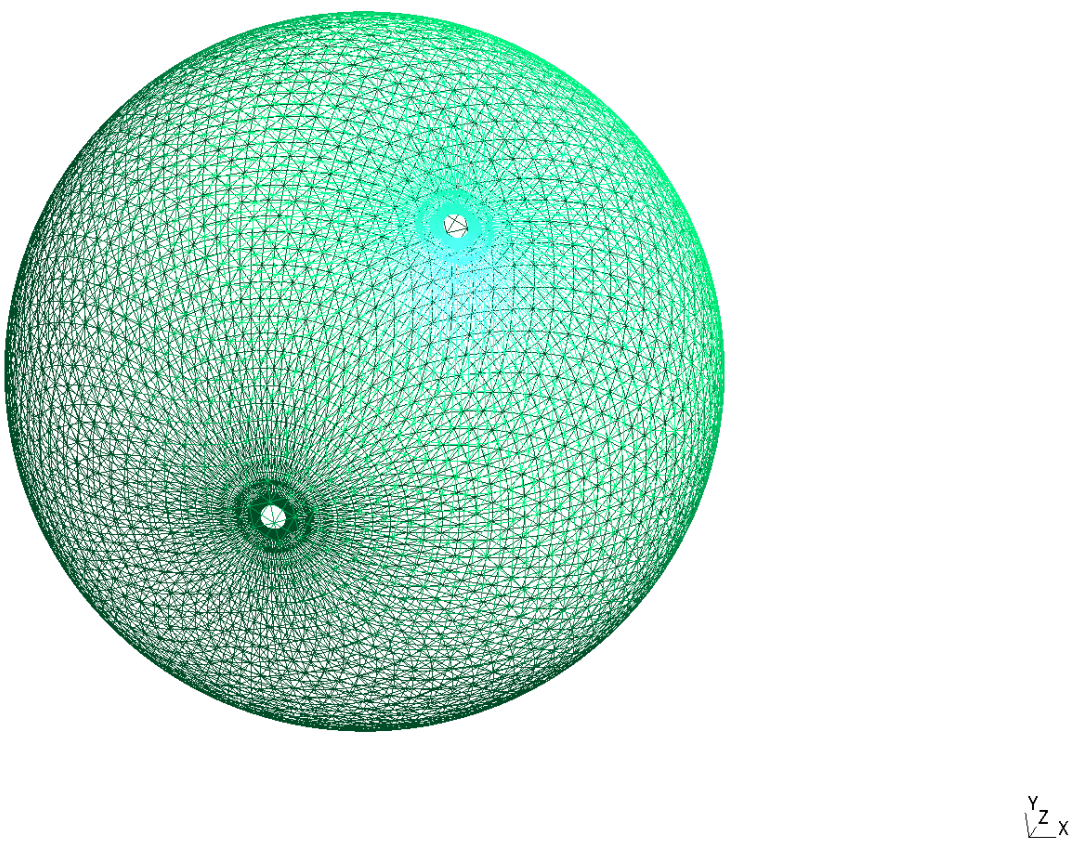
\includegraphics[width=0.95\textwidth]{imgs/Gaussian_3d}
    \caption{Three-dimensional representation of the Gaussian mesh.}
    \label{fig:section2-Gaussian-3d}
\end{figure}
%
We can now re-run the executable but, this time, using the following
command-line arguments:
%
\begin{lstlisting}[style=BashStyle]
./atlas_c-section2-Gaussian mesh2d 2
\end{lstlisting}
% 
This will generate a two-dimensional representation of the mesh.
If everything went smoothly, the mesh should look like in Fig. 
\ref{fig:section2-Gaussian-2d}.
%
\begin{figure}[H]
  \centering
    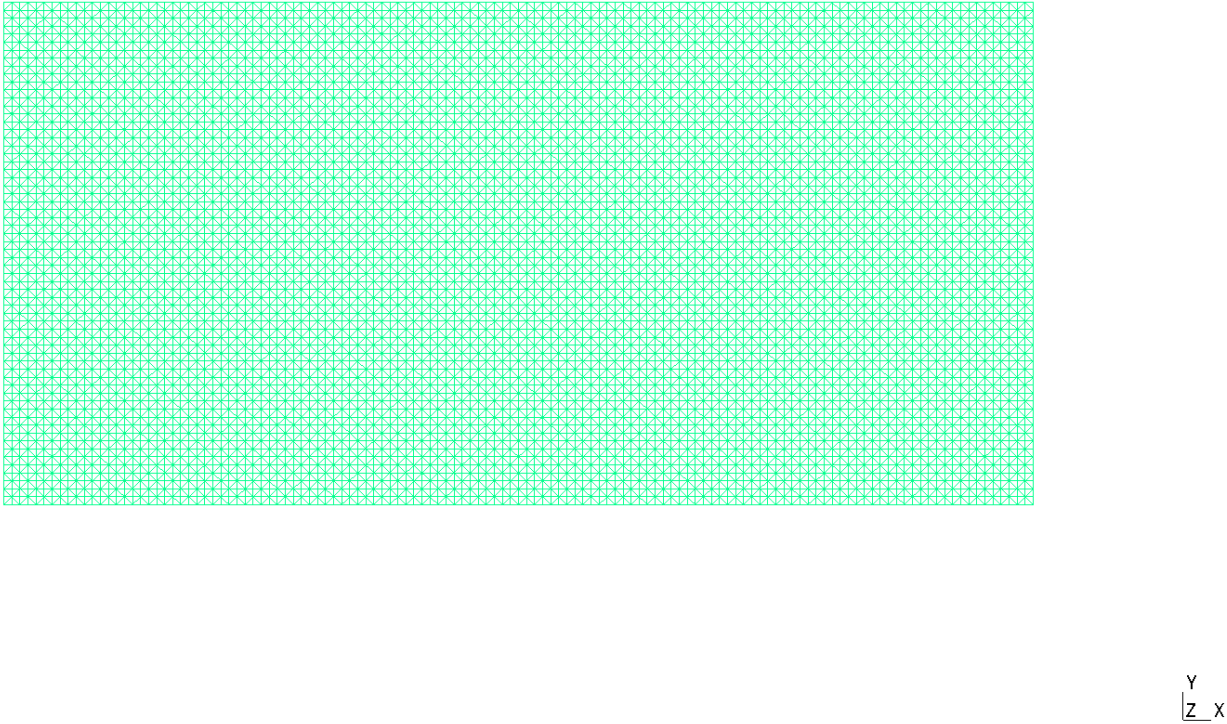
\includegraphics[width=0.95\textwidth]{imgs/Gaussian_2d}
    \caption{Two-dimensional representation of the Gaussian mesh.}
    \label{fig:section2-Gaussian-2d}
\end{figure}
%


\subsection{Reduced Gaussian Grid}
A reduced Gaussian grid is a generalisation of a Gaussian grid. 
In this case, in fact, the longitudinal and latitudinal direction
are defined independently. \textcolor{red}{In particular it is 
necessary to define a vector containing the coordinates of the 
longitudes at the equator. The longitudes at the different latitude 
levels are then computed automatically, becoming coarser while 
approaching the poles.}

Therefore, there exist some pre-loaded grids containing already 
the vector of latitudes. 

The code to generate a reduced Gaussian grid is reported in 
Listing \ref{code-2-reducedGaussian-C}.
%
\lstinputlisting[caption=Generating a reduced Gaussian grid with \Atlas 
using C++, style=CStyle, label=code-2-reducedGaussian-C]{section2-reducedGaussian.cc}
%
We note how this code is very similar to the one showed for the 
Gaussian grid. The only difference is effectively in the grid 
generation:
%
\begin{lstlisting}[style=CStyleNoLine]
Grid::Ptr RGgridPtr32(Grid::create("N32"));
\end{lstlisting}
%
In this case the constructor call a default grid called \inltc{N32},
with the vector of the latitudes being predefined. The other steps 
are exactly identical to the Gaussian grid and they are not explained 
here.

The code in Listing \ref{code-2-reducedGaussian-C}, once compiled, 
generates an executable file called \\ 
\inlsh{atlas\_c-section2\_reducedGaussian} which can be found in:
%
\begin{lstlisting}[style=BashStyle]
atlas/docs/user-guide/section2/reducedGaussian/
\end{lstlisting}
% 
\begin{notebox}
If you have compiled the documentation, you automatically have 
the executable file just mentioned without the need of doing 
any additional step.
\end{notebox}
%
We can now run the executable file with two additional command-line 
arguments, the name of the mesh file we will receive in output and 
the number of dimensions (2 or 3) we want our mesh to be generated:
%
\begin{lstlisting}[style=BashStyle]
./atlas_c-section2-Gaussian mesh3d 3
\end{lstlisting}
% 
This will create two files: \inltc{mesh3d} and \inltc{mesh3d\_info}, 
where the first file is the mesh in Gmsh format and can be opened 
in Gmsh, while the second file is a text file containing some useful 
associated to the mesh.
If everything went correctly, we should have obtained a mesh like 
the one depicted in Fig. \ref{fig:section2-reducedGaussian-3d}.
%
\begin{figure}[H]
  \centering
    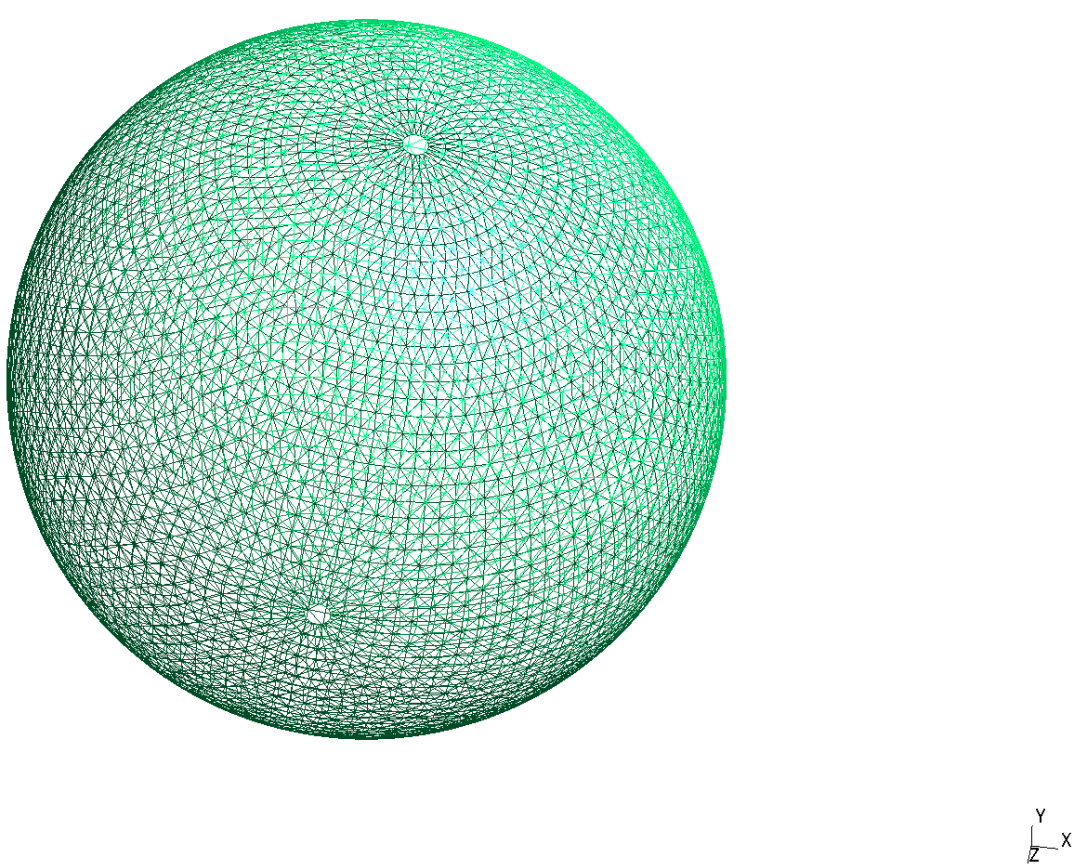
\includegraphics[width=0.95\textwidth]{imgs/reducedGaussian_3d}
    \caption{Three-dimensional representation of the reduced Gaussian mesh.}
    \label{fig:section2-reducedGaussian-3d}
\end{figure}
%
We can now re-run the executable but, this time, using the following
command-line arguments:
%
\begin{lstlisting}[style=BashStyle]
./atlas_c-section2-reducedGaussian mesh2d 2
\end{lstlisting}
% 
This will generate a two-dimensional representation of the mesh.
If everything went smoothly, the mesh should look like in Fig. 
\ref{fig:section2-reducedGaussian-2d}.
%
\begin{figure}[H]
  \centering
    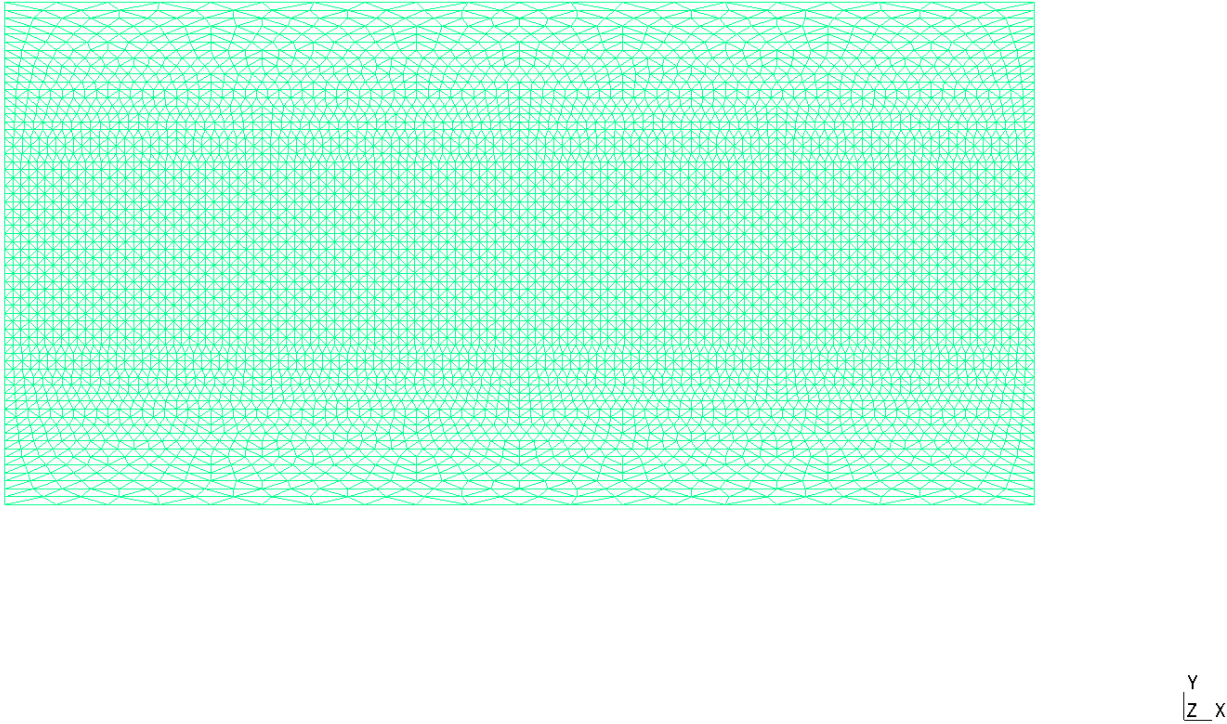
\includegraphics[width=0.95\textwidth]{imgs/reducedGaussian_2d}
    \caption{Two-dimensional representation of the reduced Gaussian mesh.}
    \label{fig:section2-reducedGaussian-2d}
\end{figure}
%
We note how in this case the longitudinal discretization in proximity 
to the poles becomes coarser.
 



\section{Fortran version}